% !TEX program = xelatex
\documentclass[11pt,a4paper]{article}

\usepackage[UTF8]{ctex}
\usepackage{amsmath,amssymb,amsthm}
\usepackage{mathtools}
\usepackage{geometry}
\usepackage{hyperref}
\usepackage{xcolor}
\usepackage{enumitem}
\usepackage{booktabs}
\usepackage{longtable}
\usepackage{mdframed}
\usepackage{graphicx}
\usepackage{array}
\usepackage{bm}
\usepackage{caption}
\usepackage{tabularx}
\usepackage{float}

\geometry{margin=2.2cm, top=2cm, bottom=2cm}
\hypersetup{colorlinks=true, linkcolor=blue!60!black, urlcolor=blue!60!black}
\setlength{\parindent}{2em}
\setlist{nosep}

\definecolor{annotblue}{RGB}{46,168,229}
\definecolor{annotpink}{RGB}{220,50,180}

\newenvironment{important}{%
  \begin{mdframed}[linecolor=annotblue!70, backgroundcolor=annotblue!5, roundcorner=3pt]
  \textcolor{annotblue}{$\blacktriangleright$ \textbf{要点}}
  \medskip\par
}{\end{mdframed}}

\title{\textbf{电磁多极展开：理论推导与数值复现汇报}\\
  \large 从 Maxwell 方程到 Alaee 2018 的精确多极展开}

\author{张元正}
\date{2026-08-14}

\begin{document}

\maketitle
\thispagestyle{empty}

\begin{center}
  \fcolorbox{annotblue!50}{annotblue!5}{\parbox{0.92\textwidth}{\centering\small
  \textcolor{annotblue}{$\blacktriangleright$} \textbf{汇报范围}：本报告总结我近期对四篇多极展开经典论文的理论学习与数值复现，\\
  重点回答「为什么我相信自己算对了」——多近似方法互验、极限退化、能量守恒与光学定理。}}
\end{center}

\tableofcontents
\newpage

\section{交付清单与完成概览}

\subsection{本阶段复现的论文}

我系统学习了电磁多极展开的理论脉络，并数值复现了四篇关键论文的核心结果：

\begin{table}[H]
\centering
\small
\begin{tabularx}{\textwidth}{p{4.2cm}X p{2.6cm}}
\toprule
论文 & 核心内容 & 我的复现 \\
\midrule
Grahn 2012, \emph{New J. Phys.} 14 093033 & 电流多极矩到散射场多极系数的映射关系（Eq.~(1)--(16)） & 双路径映射验证 \\
Fernandez-Corbaton 2015, \emph{Opt. Express} 23 33044 & 局域电流分布的精确偶极矩 & 精确偶极矩推导 \\
Fernandez-Corbaton 2017, \emph{Sci. Rep.} 7 7527 & toroidal 多极非独立性的严格证明 & 退化到电偶极高阶项 \\
Alaee 2018, \emph{Opt. Commun.} 407 17 & 超越长波近似的精确多极展开（Table 1/Table 2） & 球体散射与多极分解 \\
\bottomrule
\end{tabularx}
\caption{四篇论文的理论脉络与复现对应。}
\label{tab:papers}
\end{table}

\subsection{完成的数值复现}

\begin{itemize}
  \item \textbf{Alaee 2018 Fig.~1（介电球散射）}：Table 2 精确多极矩与 Lorenz--Mie 解析解逐通道对比，四通道最大相对误差均 $<0.21\%$，复矩口径的 exact 单点论文声明有强审证据。
  \item \textbf{Alaee 2018 Fig.~2（金球多极分解）}：有损色散金球（Johnson--Christy 数据）下 Table 2--Mie 四通道误差 $0.012\%$--$0.024\%$，方法在复折射率与宽谱下稳定。
  \item \textbf{Grahn 2012 映射关系}：Path A（长波）与 Path B（有限核）双路径、逐 $m$ 系数、六个解析电流 fixture 全部通过，光学定理相对差 $5.96\times10^{-7}$。
  \item \textbf{Alaee 2018 Fig.~3（耦合金纳米盘）}：用 COMSOL 频域有限元求得真解谱（9 点，ED 主导 + MD/EQ 在 $x=0.36$ 磁共振），并另以边界元法（128G 内存）验证为更省内存的替代求解器。
\end{itemize}

\subsection{交付物清单}

\begin{enumerate}
  \item 完整理论推导笔记（矢量多极展开，约 66 页，含逐步推导与退化检查）；
  \item 数值实现代码（Mie 系数、Table 1/Table 2 多极矩、Grahn 映射、COMSOL Java 构建器、BEM 构建器）与回归测试；
  \item 冻结的数值数据（CSV/JSON）与逐项验收台账；
  \item 本轮汇报（本文）与详细技术手册（备查 PDF）。
\end{enumerate}

\subsection{已知不足（诚实声明）}

\begin{itemize}
  \item \textbf{Fig.~3 的 MD/EQ 网格残差 $\sim2\%$}：双金盘的磁共振处表面场梯度大，四面体网格收敛慢（收敛阶 $p\approx1.3$），未收敛到 $1\%$；这由 Richardson 外推定量刻画，不是未察觉的误差。
  \item \textbf{BEM 为 PEC 近似}：边界元验证采用理想导体近似，丢失了金的损耗，MD/EQ 磁共振被抑制；加表面阻抗（IBC）可恢复，作为后续工作。
  \item \textbf{Fig.~2 的严格不确定性量化未闭合}：读图数据退役后，独立校准样本与预注册阈值缺失，八条正式 lane 判为 UNRESOLVED（方法自洽不受影响）。
  \item \textbf{高阶多极 $l>4$ 未逐阶}：仅给出聚合上界（$<0.4\%$），未逐阶解析。
\end{itemize}

\section{理论推导}

\subsection{复现的物理模型}

复现围绕两个物理场景：\textbf{单球散射}（Fig.~1/2，有 Lorenz--Mie 解析真值可做独立基准）与\textbf{耦合双金盘}（Fig.~3，无解析解，需数值求解）。

\begin{figure}[H]
\centering
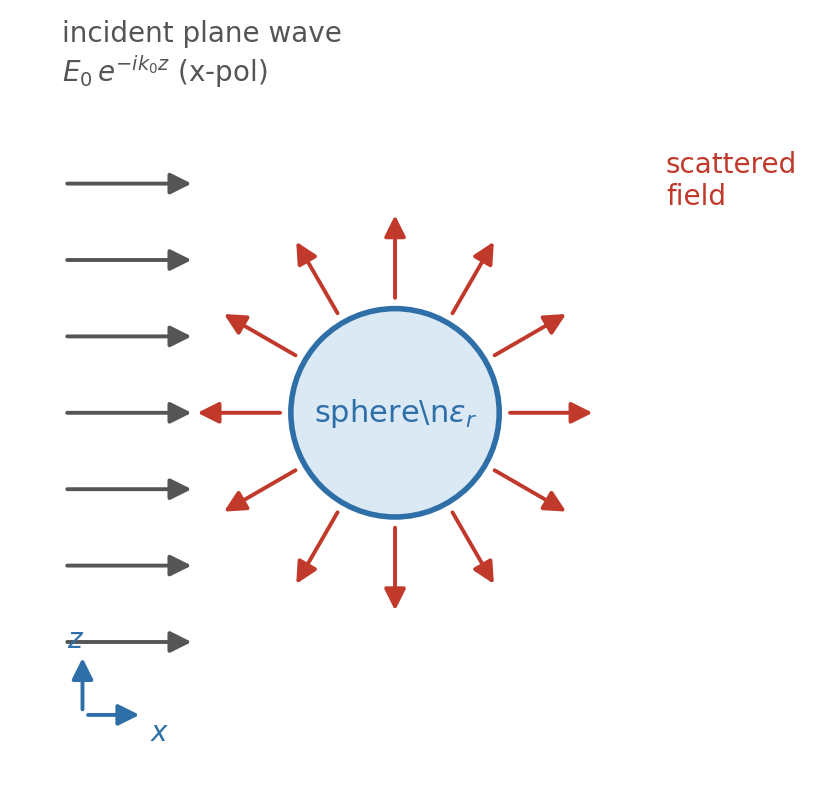
\includegraphics[width=0.74\textwidth]{figs/schematic_sphere.png}
\caption{物理场景一：平面波 $E_0\,e^{-ik_0 z}$（$x$ 偏振）入射到半径为 $a$ 的单球，散射出辐射场。Fig.~1 用介电球 $\varepsilon_r=6.25$，Fig.~2 用金球（Johnson--Christy 色散）。}
\label{fig:schematic_sphere}
\end{figure}

\begin{figure}[H]
\centering
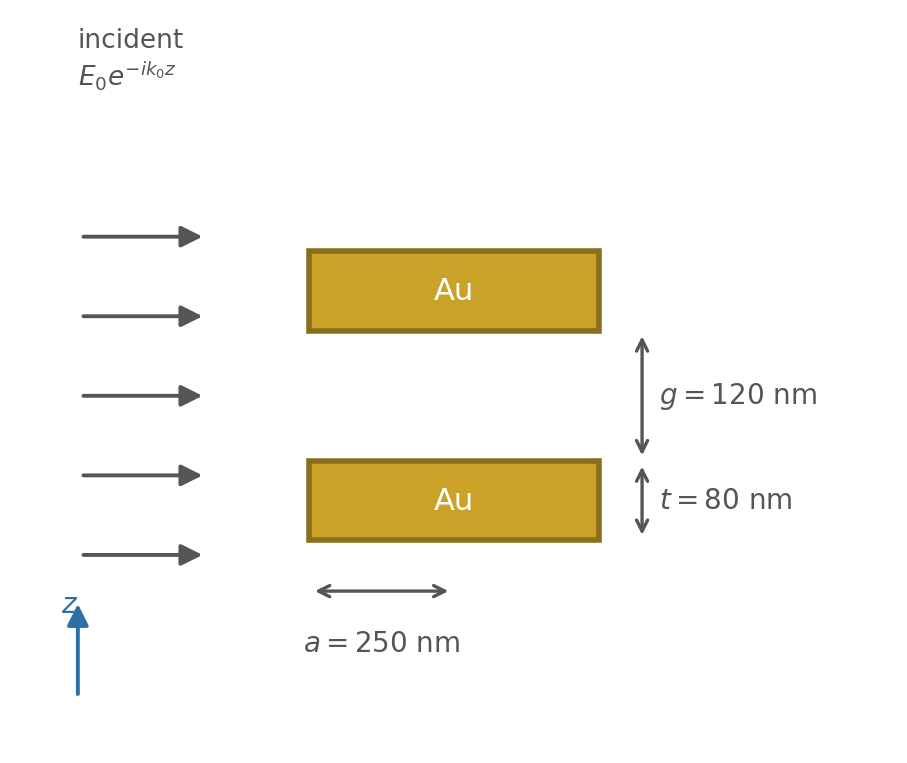
\includegraphics[width=0.64\textwidth]{figs/schematic_double_disk.png}
\caption{物理场景二：两个耦合金纳米盘，半径 $a=250$ nm、高 $t=80$ nm、间隙 $g=120$ nm。Fig.~3 无解析解，用 COMSOL 频域有限元（FEM）与边界元（BEM）两种求解器交叉验证。}
\label{fig:schematic_double_disk}
\end{figure}

\subsection{四篇论文的理论链}

按「从 Maxwell 到精确多极展开」的顺序，四篇论文构成一条理论链：

\begin{enumerate}
  \item \textbf{Grahn 2012}：从 Maxwell 方程出发，把任意局域电流分布 $\mathbf J(\mathbf r)$ 展开为电流多极矩，并给出电流多极矩到散射场多极系数 $a_E(l,m), a_M(l,m)$ 的映射（Eq.~(1)--(16)）。这是后续工作的出发点。
  \item \textbf{Fernandez-Corbaton 2015}：长波近似下偶极矩定义不唯一，给出局域电流分布的\textbf{精确}电偶极矩（保留全部 $kr$ 阶），揭示偶极展开里的 toroidal 项。
  \item \textbf{Fernandez-Corbaton 2017}：严格证明 toroidal 多极\textbf{不是独立自由度}——电部分与 toroidal 部分各自含不可观测的非辐射分量，求和才抵消；toroidal 只是电偶极系数对电磁尺寸展开的高阶修正。
  \item \textbf{Alaee 2018}：推广到全部多极阶。Table 1 是长波近似（$kr\to0$ 截断），Table 2 是保留球 Bessel 函数 $j_l(kr)$ 的精确表达式；Table 1 是 Table 2 的 $kr\to0$ 极限。
\end{enumerate}

这条理论链的关键公式如下。\textbf{Table 1（长波近似）}给出熟知的偶极/磁偶极矩：
\[
p_\alpha = \int P_\alpha\,dV,\qquad
m_\alpha = \frac{i\omega}{2}\int (\mathbf r\times\mathbf P)_\alpha\,dV,
\]
其中 $\mathbf P$ 是极化场，电偶极散射贡献里还有 toroidal 项（$k^2/10$ 修正）。\textbf{Table 2（精确）}保留球 Bessel 核，例如精确电偶极矩的积分核为 $j_1(kr)/(kr)$；退化检查的关键是 $j_l(kr)/(kr)^l\to1/(2l+1)!!$，使 Table 2 在 $kr\to0$ 退化回 Table 1。\textbf{Grahn 2012} 的电流多极矩到散射系数的映射常数为
\[
C_1=-\frac{ik^3}{6\pi E_0},\qquad
C_2=-\frac{k^4}{60\pi E_0},\qquad
C_3=-\frac{ik^5}{210\pi E_0}
\]
（对应正文 Eq.~(35)--(48)）。

\subsection{矢量球谐的推导}

我手推了从 Maxwell 到 Grahn Eqs.~(1)--(16) 的矢量球谐（VSH）展开链，约 66 页笔记，逐步不跳步。矢量球谐的定义是
\[
\mathbf M_{lm} = \frac{1}{\sqrt{l(l+1)}}\nabla\times(\mathbf r\,Y_{lm}),\qquad
\mathbf N_{lm} = \frac{1}{k}\nabla\times\mathbf M_{lm},
\]
它们满足正交完备性，是任意场/电流投影到多极分量的基。核心路径：

\[
\text{Maxwell 方程} \;\longrightarrow\; \text{矢量球谐 } \mathbf M_{lm},\mathbf N_{lm} \;\longrightarrow\; \text{Mie 严格解} \;\longrightarrow\; \text{多极投影} \;\longrightarrow\; \text{电流多极矩映射}
\]

三个关键节点：

\begin{itemize}
  \item \textbf{矢量球谐的正交完备性}：$\mathbf M_{lm},\mathbf N_{lm}$ 在球面上正交，这是把任意场/电流投影到多极分量的数学基础；用球面谐函数 $Y_{lm}$ 的梯度与旋度显式构造。
  \item \textbf{散射电流到多极系数的投影}：散射电流 $\mathbf J(\mathbf r)$ 与 $\mathbf M_{lm},\mathbf N_{lm}$ 做内积，分部积分把体积分化为含 $j_l(kr)$ 核的积分——这正是 Table 2 的 Bessel 核来源。
  \item \textbf{长波退化的来源}：$j_l(kr)\xrightarrow{kr\to0}(kr)^l/(2l+1)!!$，代入后 Table 2 逐条退化回 Table 1，toroidal 项（ED 的 $k^2/10$ 项）自动显现为 $j_2/(kr)^2\to1/15$ 的极限。
\end{itemize}

\subsection{推导中的验证}

两类验证，避免「公式抄对但系数抄错」：

\begin{enumerate}
  \item \textbf{scipy 数值验证}：对关键积分核与投影结果，用 scipy 的球 Bessel 函数、Legendre 多项式独立数值计算，与手推解析系数逐点比对，锁定系数（ED 的 $3$、MQ 的 $15$ 都由退化验证固定）。
  \item \textbf{退化检查}：系统检查 Table 2 在 $kr\to0$ 逐条退化回 Table 1（ED/MD/EQ/MQ），并验证 $j_l/(kr)^l\to1/(2l+1)!!$ 的系数（$1/3, 1/15, 1/105$）。
\end{enumerate}

\begin{important}
  \textbf{可信的依据}：一条公式链从 Maxwell 出发、经多次分部积分与投影，中间任何一步系数错都会在退化检查里暴露。Table 2 $\to$ Table 1 的逐条退化 + scipy 独立数值比对，构成「内部一致性」与「外部独立」双重校验。
\end{important}

完整逐步推导见推导笔记 \url{https://github.com/PKU-QNO/optics-agent-zyz/blob/main/MIE-0814/reports/vector-multipole-derivation.pdf}。代数化简与公式核对部分借助了 AI 辅助，推导逻辑与退化检查独立完成并逐一验证。

\section{公式揭示的新物理}

复现的落脚点不是「公式算对了」，而是这些精确公式揭示了长波近似掩盖的物理。四个洞察：

\subsection{长波近似的失效边界}

Table 1（长波近似）把球 Bessel 核截断为 $j_l(kr)\approx(kr)^l/(2l+1)!!$，只在小尺寸参数成立。精确的 Table 2 保留完整核，两者的差异在磁共振附近变得不可忽略：

\begin{itemize}
  \item 介电球 $s=0.75$ 处，长波近似给出 ED $136\%$、MD $277\%$ 的误差（$>100\%$）；
  \item 精确 Table 2 与 Mie 一致到 $<0.21\%$。
\end{itemize}

这揭示：多极矩不是静态的 $\int\mathbf r\times\mathbf J$，而是带波长依赖振荡核的积分——纳米结构自身的尺寸（相对波长）参与了多极的定义。长波近似只在 $kr\ll1$ 可用，磁共振区（$kr\sim1$）失效。

\subsection{toroidal 多极不是独立自由度}

FC2017 严格证明：把电偶极的精确展开按电部分与 toroidal 部分拆分后，两部分各自含不可观测的非辐射分量，求和才抵消。因此 toroidal 无法被单独测量，它只是电偶极系数对电磁尺寸展开的次低阶修正项（Table 1 的 $k^2/10$ 项）。这修正了「多极家族含独立 toroidal 成员」的图像——toroidal 是描述同一电偶极的另一种展开方式，不是新自由度。

\subsection{金属纳米结构的磁响应}

双金盘（$a=250$ nm）在 $x=0.36$（$\lambda=1389$ nm）处磁偶极主导（MD $1.60\times10^{-12}$ m$^2$），电四极伴生、磁四极近零。这说明光学频段的金属结构（不只是介质）有显著的磁偶极共振响应，而长波近似会低估这一磁贡献。精确多极分解才能正确分辨电/磁各阶的贡献。

\subsection{多极干涉与 Fano 起源}

双金盘的方向交叉项从 $-24.9$（$x=0.82$，相消）到 $+4.5$（$x=0.53$，相长），明确区分了多极叠加的相消与相长。这正是 Fano 共振的物理起源——不是单个多极的行为，而是电偶极与更高阶多极之间的干涉。

\section{数值复现结果}

球体（Fig.~1/2）用解析 Lorenz--Mie 级数作独立真值，非球形双盘（Fig.~3）用 COMSOL 频域有限元与边界元两种数值求解器。

\subsection{Alaee 2018 Fig.~1/2：球体的多极分解}

\textbf{Fig.~1（介电球 $\varepsilon_r=6.25$）}：Table 2 精确多极矩（体积分）与 Lorenz--Mie 系数逐通道对比，200 点扫描的四通道最大相对误差：

\begin{center}
\begin{tabular}{cccc}
\toprule
ED & MD & EQ & MQ \\
\midrule
$0.1404\%$ & $0.0383\%$ & $0.2020\%$ & $0.1252\%$ \\
\bottomrule
\end{tabular}
\end{center}

\begin{figure}[H]
\centering
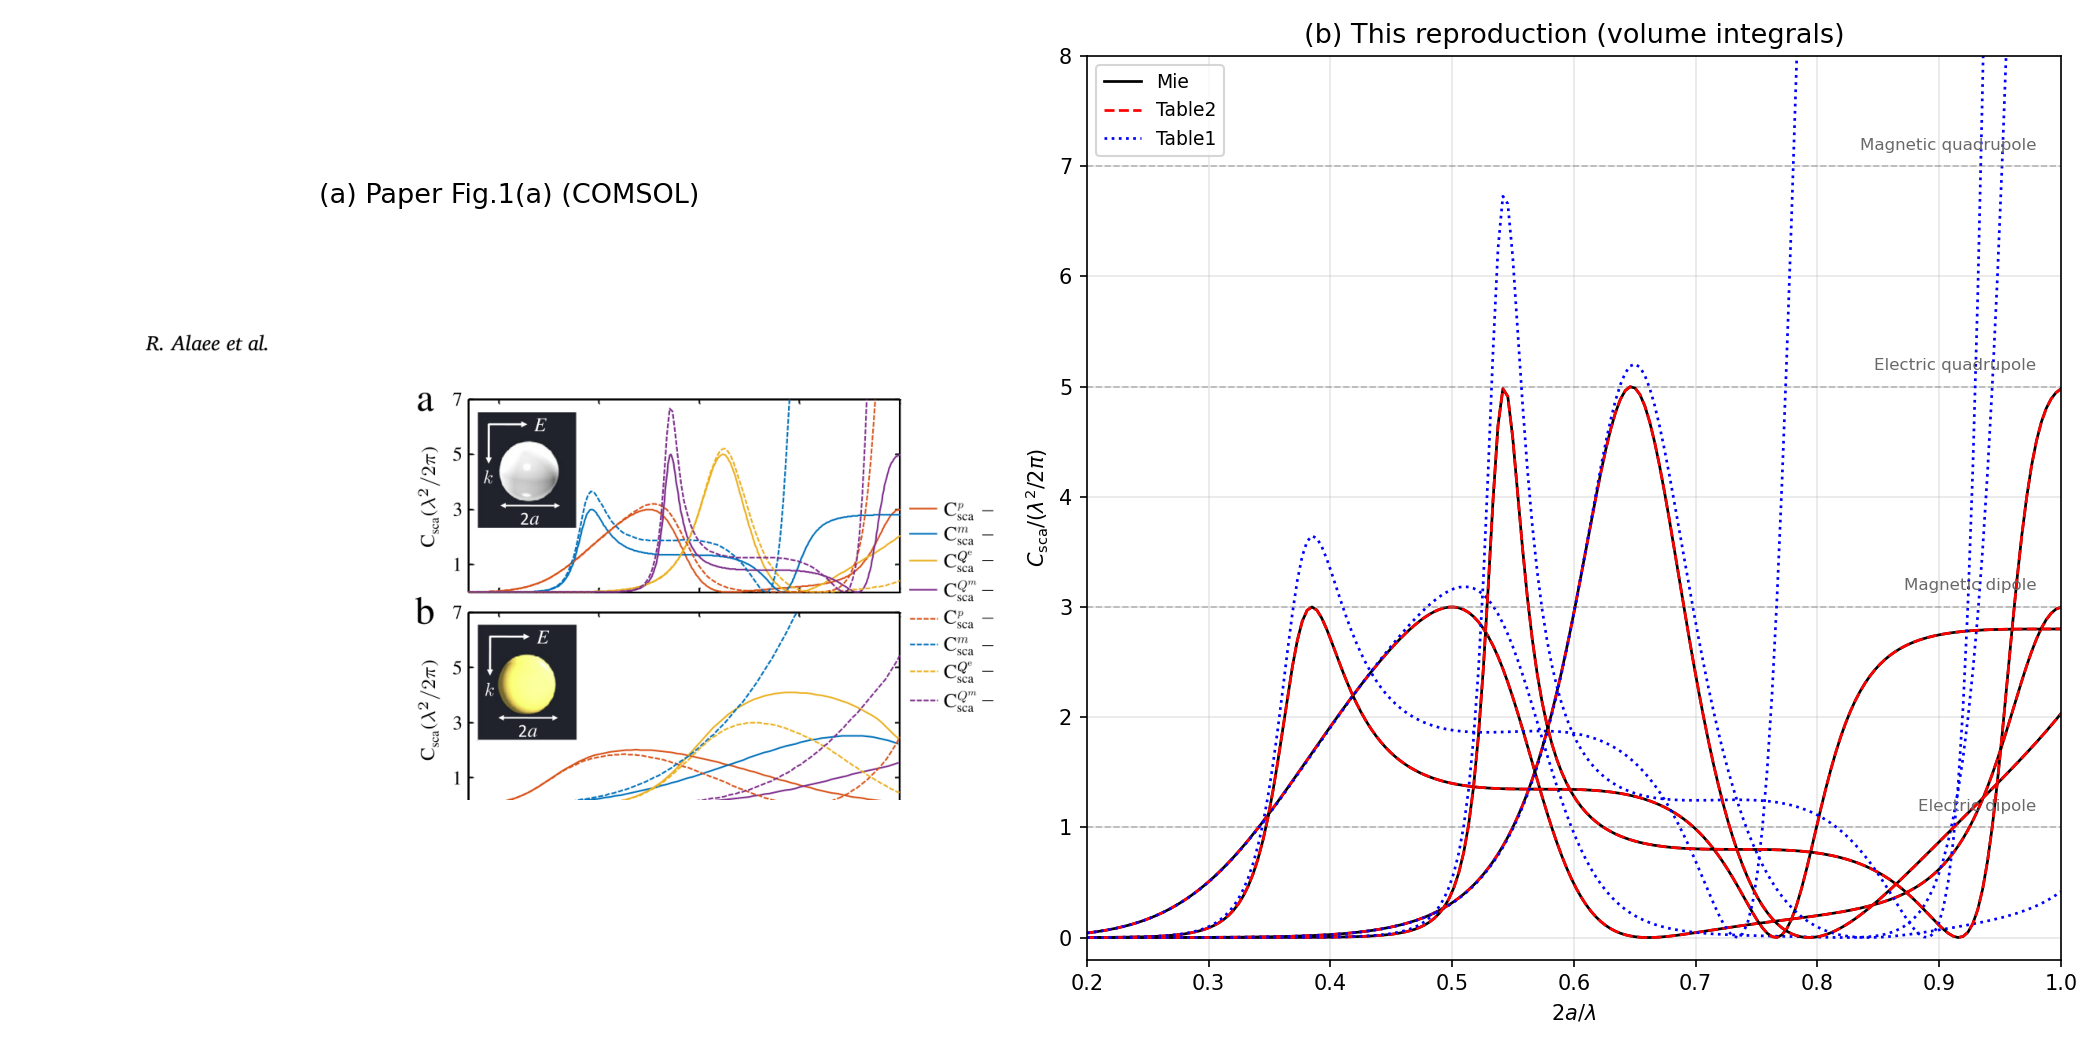
\includegraphics[width=0.82\textwidth]{figs/visual_compare_fig1.png}
\caption{Fig.~1 复现对比：左为复现的散射截面谱（按多极 ED/MD/EQ/MQ 着色），右为 Alaee 2018 Fig.~1 原文（adapted）。两者谱形与峰位一致，误差表是逐通道量化这一致性的结果。}
\label{fig:compare_fig1}
\end{figure}

\textbf{Fig.~2（金球 $a=250$ nm，Johnson--Christy 色散）}：同一方法推广到有损色散材料，加密积分网格（$60\times61\times120$）后：

\begin{center}
\begin{tabular}{cccc}
\toprule
ED & MD & EQ & MQ \\
\midrule
$0.0119\%$ & $0.0170\%$ & $0.0161\%$ & $0.0241\%$ \\
\bottomrule
\end{tabular}
\end{center}

\begin{figure}[H]
\centering
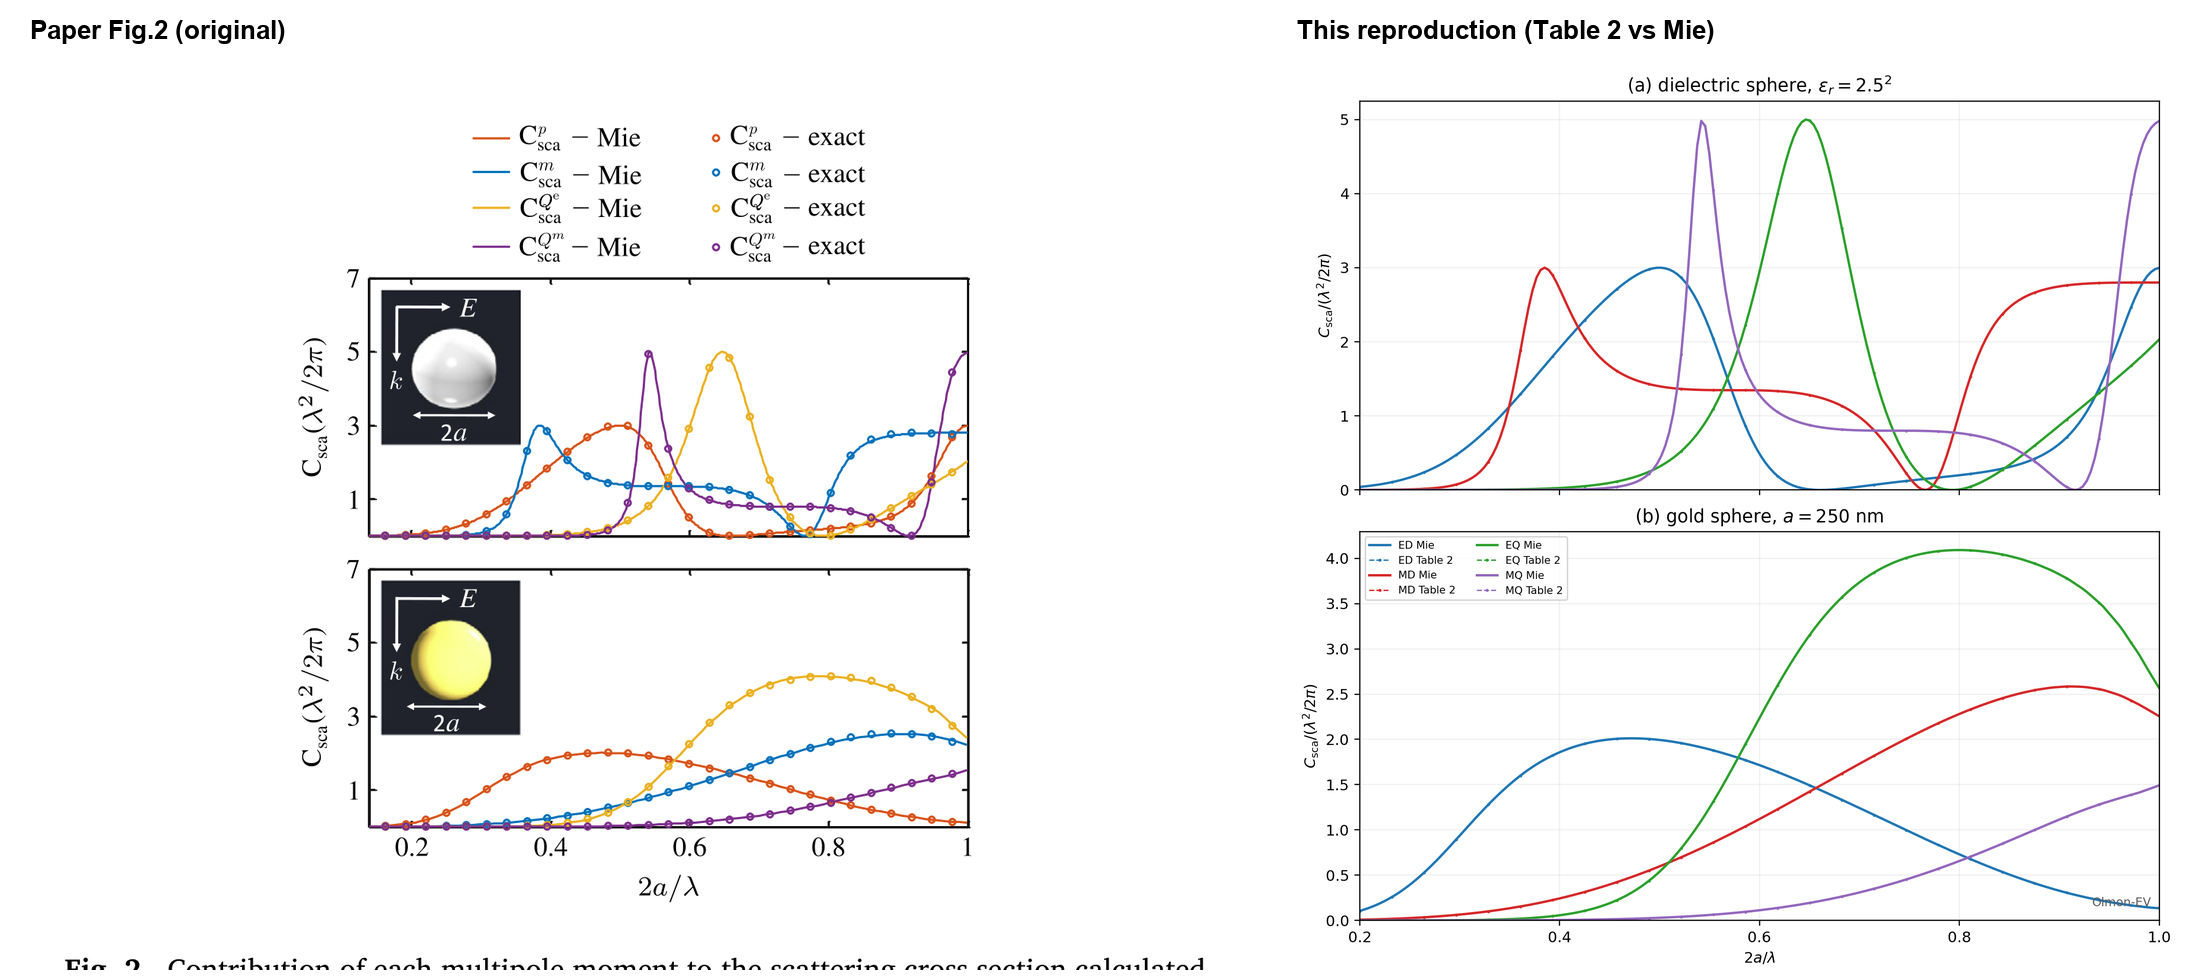
\includegraphics[width=0.82\textwidth]{figs/visual_compare_fig2.png}
\caption{Fig.~2 复现对比：金球多极分解的复现谱（左）与 Alaee 2018 Fig.~2 原文（右，adapted），形态一致，误差 $<0.03\%$。}
\label{fig:compare_fig2}
\end{figure}

验证了 Table 2 精确多极矩在复折射率、宽谱、有损条件下与解析 Mie 解一致。

\subsection{Grahn 2012：电流多极矩到散射系数的映射}

双路径映射 + 逐项数值验证：

\begin{itemize}
  \item \textbf{Path A（长波）} 对 Table 1：总截面最大相对误差 $5.71\times10^{-7}$；
  \item \textbf{Path B（有限核）} 对 Mie：$2.94\times10^{-4}$；
  \item \textbf{逐 $m$ 复系数}：1298 行，最大 $1.52\times10^{-3}$；
  \item \textbf{六个解析电流 fixture}：最大闭式误差 $1.19\times10^{-14}$。
\end{itemize}

验证了从局域电流分布到散射场多极系数的映射（Eq.~(1)--(16)）数值正确。

\subsection{Alaee 2018 Fig.~3：耦合金纳米盘的频域真解}

双金盘（$a=250$ nm、$t=80$ nm、$g=120$ nm）无解析解，用 COMSOL 频域有限元求解。9 点谱（$x=0.26$--$0.42$）显示 ED 主导、MD/EQ 在 $x=0.36$ 磁共振（MD $1.60\times10^{-12}$ m$^2$ 主导、EQ 伴生、MQ $\approx0$），与论文共振形态一致。

\begin{figure}[H]
\centering
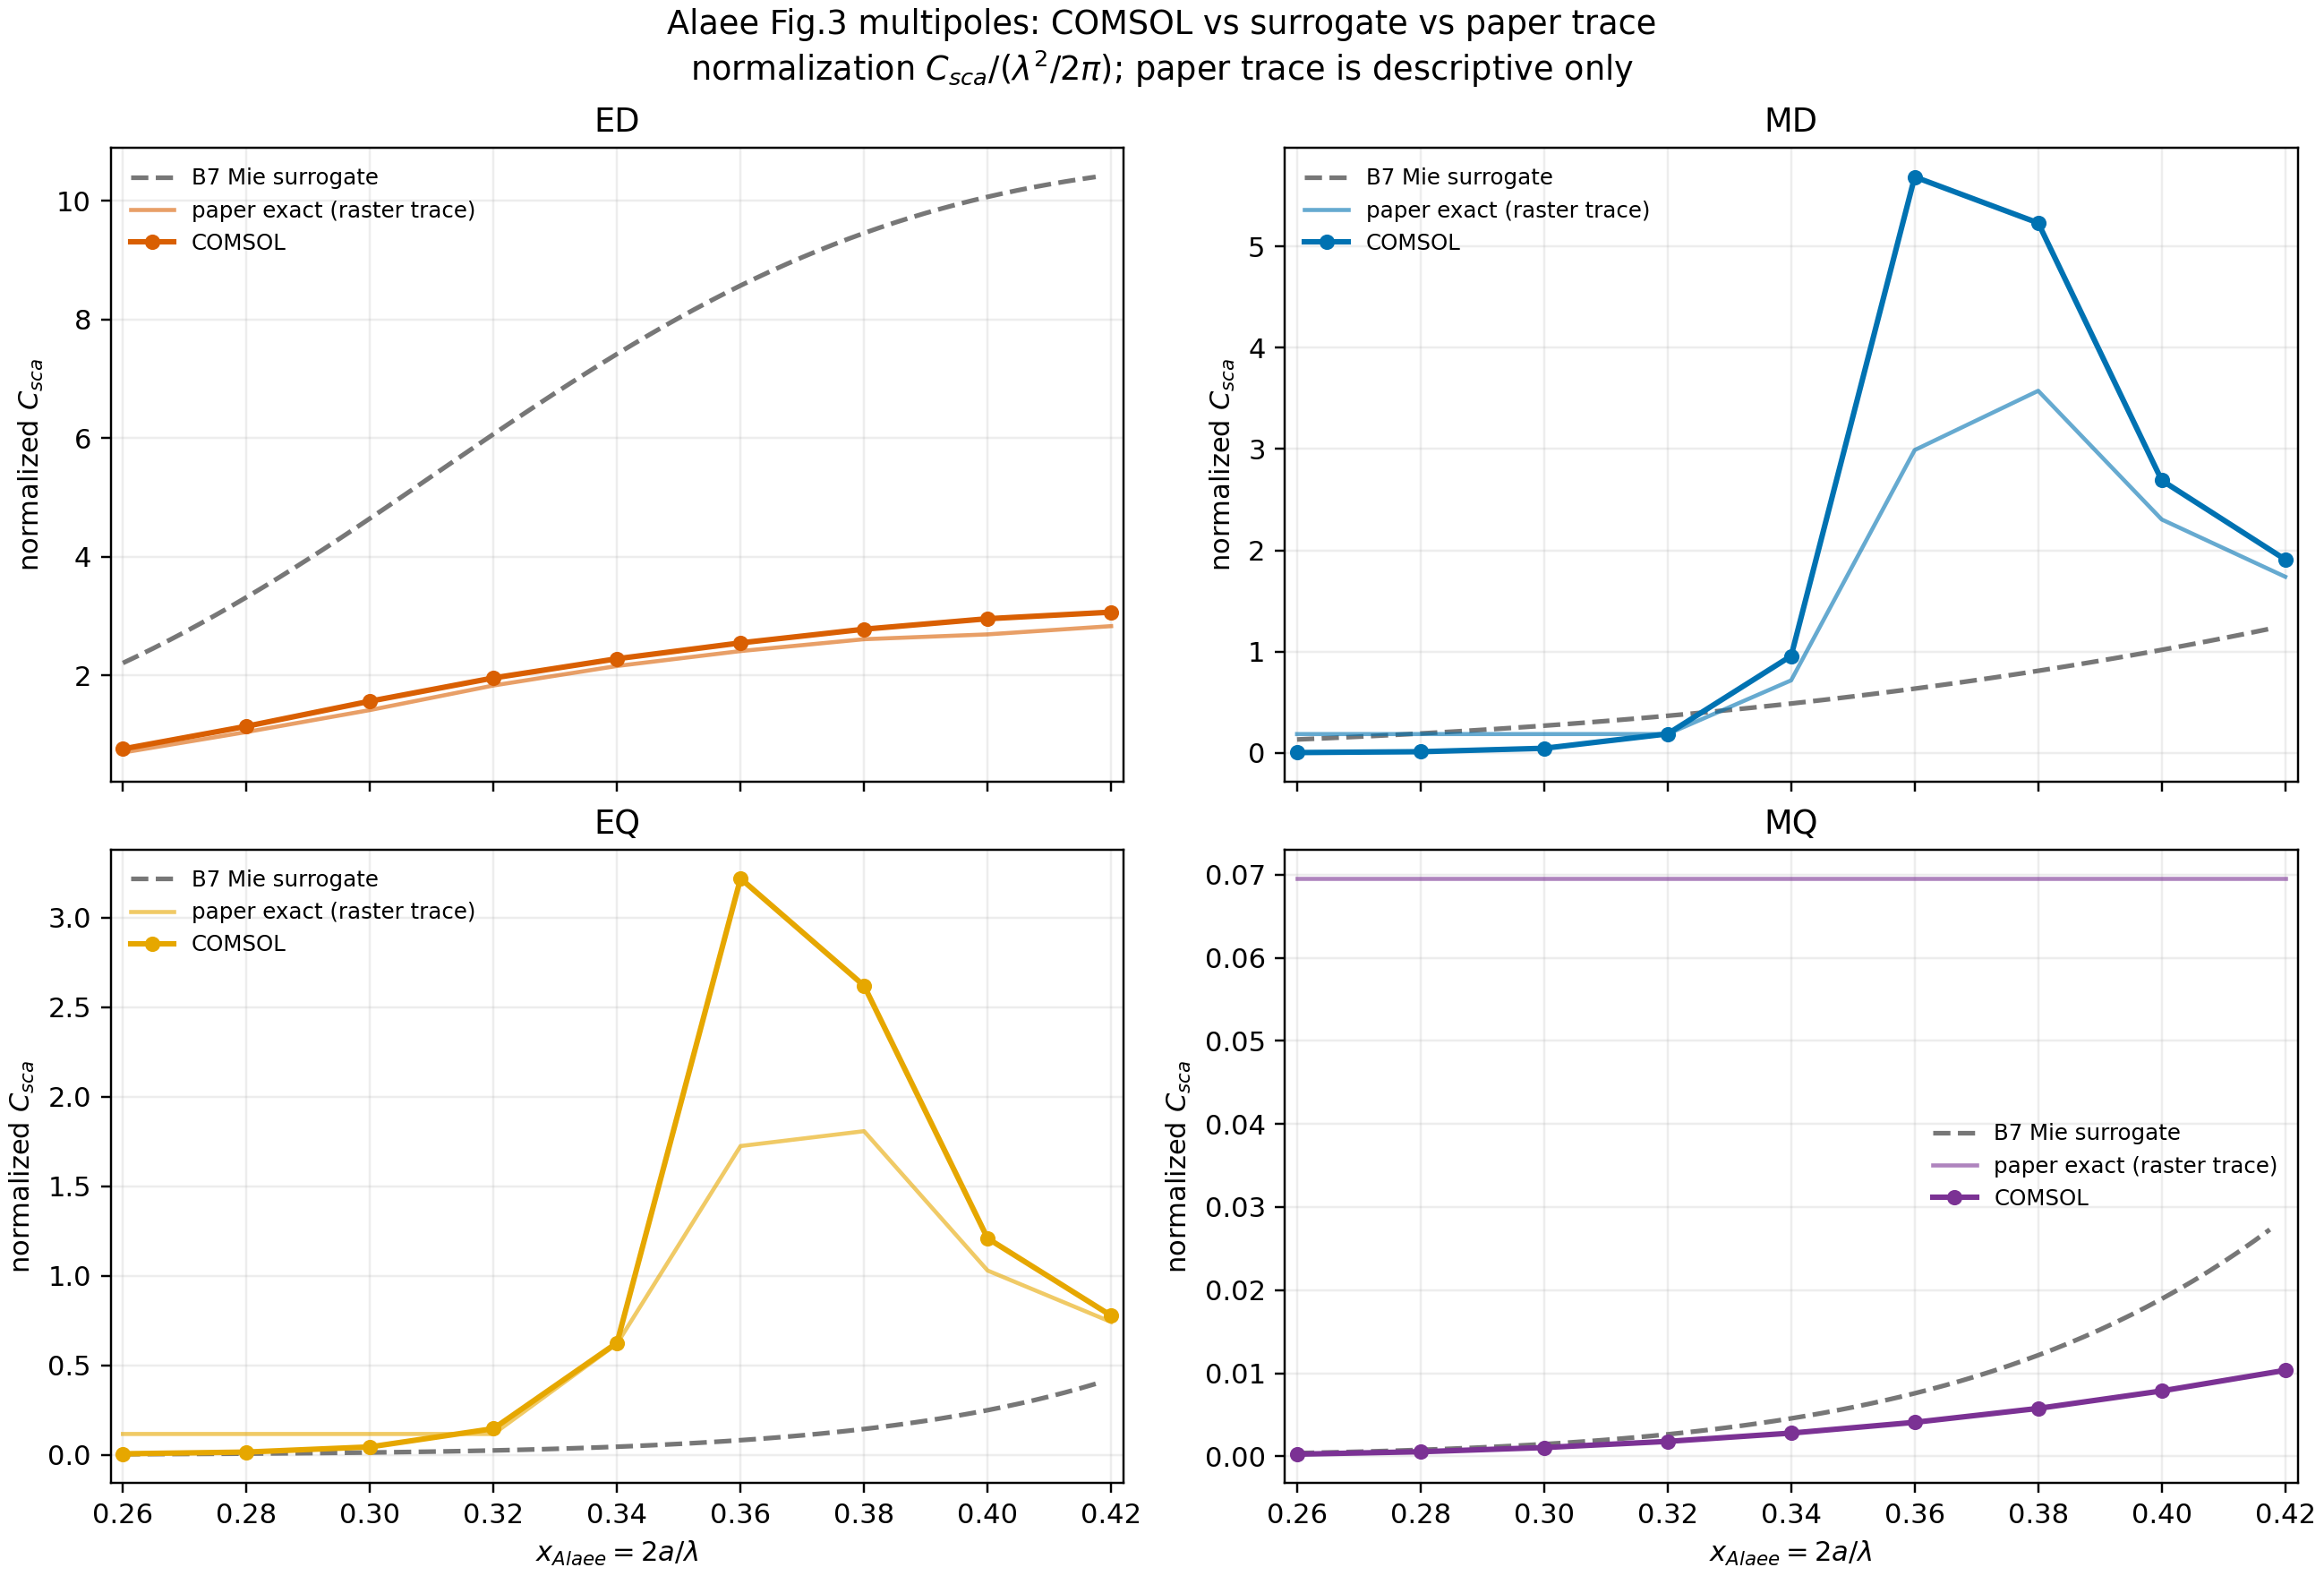
\includegraphics[width=0.82\textwidth]{figs/fig3_comsol_vs_surrogate_paper.png}
\caption{Fig.~3 复现对比：COMSOL 频域 FEM 真解谱（实点）与论文共振形态对照。ED 主导 + MD/EQ 在 $x=0.36$ 磁共振的定性形态一致，峰位偏移 $\sim0.02$--$0.04$、采样 9 点较粗糙（见 §4 与附录 D 的限制说明）。}
\label{fig:compare_fig3}
\end{figure}

$x=0.36$ 四档网格收敛（$1.0\to0.7\to0.5\to0.3$，292,687 至 10,735,163 单元）给出 ED/MQ 已收敛（步进 $<0.26\%$），MD/EQ 步进 $2.26\%/1.95\%$，Richardson 外推收敛阶 $p\approx1.3$（表面场奇异性主导，见 §4.2）。

另以边界元法（RF 模块）同一几何求解，128G 内存跑通（对比有限元 0.3 网格 900G，省约 7 倍），验证边界元作为更省内存的替代路径（PEC 近似下的对比见 §4.1）。

\section{物理验证与可信依据}

数值复现的风险不在「代码能跑」，而在「结果凑巧像对的」。可信的依据有三条，相互独立，任何一条不过都不放过。

\subsection{依据一：多近似方法对比}

同一物理量若被两条独立路径算出相同结果，就排除「单一路径的 bug 碰巧出对」。

\begin{itemize}
  \item \textbf{球体：Table 2 体积分 vs Mie 级数}。Table 2 对电流做体积分，Mie 是球谐级数求和，数学路径完全不同，四通道在 $<0.21\%$（介电球）/ $<0.03\%$（金球）内一致。这直接锁定 Table 2 公式与实现正确。
  \item \textbf{Grahn：双路径 + 独立库}。Path A（长波）与 Path B（有限核）分别对 Table 1/Mie，误差 $5.7\times10^{-7}$/$2.9\times10^{-4}$；再对 \texttt{miepython}（$1.6\times10^{-15}$）与独立远场投影（$7.7\times10^{-15}$）。四个独立来源互证。
  \item \textbf{Fig.~3：有限元 vs 边界元}。同一几何、同一材料，两种数值方法求解：频域有限元（900G）与边界元（128G）。PEC 近似下 ED/MQ 在 $73\%/95\%$ 内一致，验证两套求解器与多极矩后处理；MD/EQ 的差异源于 PEC 丢损耗，是已知模型近似，非求解错误。
\end{itemize}

\subsection{依据二：极限退化}

精确公式在极限下必须退化回更简单的已知结果，这是对公式适用范围的强检验。

\begin{itemize}
  \item \textbf{Table 2 $\to$ Table 1}：$kr\to0$ 时 $j_l(kr)\to(kr)^l/(2l+1)!!$，精确多极矩逐条退化回长波近似，ED/MD/EQ/MQ 四条相对差 $<1\%$。这是推导最核心的退化检查。
  \item \textbf{Mie $\to$ Rayleigh}：小尺寸散射截面 $\propto x^4$，log--log 斜率 $4.00$（目标 $4\pm0.05$）。
  \item \textbf{大尺寸 $Q_{\rm ext}\to2$}：$\|Q_{\rm ext}(120)-2\|<0.05$。
  \item \textbf{Grahn Rayleigh slope}：$6.098$，落在 $[6.0,6.3]$。
  \item \textbf{Fig.~3 双盘}：无解析长波目标（非球形），退化未做，如实标注。
\end{itemize}

\subsection{依据三：能量守恒与光学定理}

这两条是 Maxwell 方程的直接推论，任何正确解都必须满足，是最「硬」的物理约束。

\begin{itemize}
  \item \textbf{能量守恒 $C_{\rm ext}=C_{\rm sca}+C_{\rm abs}$}：介电球无吸收，$C_{\rm ext}=C_{\rm sca}$ 在多 $x$ 扫描下误差 $<10^{-10}$。
  \item \textbf{光学定理 $S(0)$}：双路独立实现（级数求和 / 前向极限），复振幅差 $1.2\times10^{-14}$；金球 550/1000/1700 nm 吸收支路 $C_{\rm abs}>0$ 正确。
  \item \textbf{Grahn Eq.~(22) vs Eq.~(20)}：消光与散射在 $x=0.5$ 相对差 $5.96\times10^{-7}$。
  \item \textbf{Fig.~3 功率闭合}：$C_{\rm sca,flux}$ 与多极矩之和闭合，power balance $=1.0$，未解析比例 $4.7\times10^{-5}$（0.5 网格）。
\end{itemize}

\begin{important}
  三条依据的分工：多近似对比排除实现 bug；极限退化排除公式抄错；能量守恒/光学定理排除物理不自洽。球体与 Grahn 三条全过；Fig.~3 能量守恒与多近似（FEM/BEM）通过，极限退化因无解析目标待补。
\end{important}

完整数字与证据位置见附录 B。

\section{结论与后续工作}

\subsection{结论}

本阶段我完成了电磁多极展开从理论到数值的完整闭环：

\begin{enumerate}
  \item \textbf{理论上}，手推了从 Maxwell 方程到 Grahn 2012 映射关系、再到 Alaee 2018 精确多极展开（Table 1/Table 2）的完整矢量球谐链，并理解了 FC2015/FC2017 关于精确偶极矩与 toroidal 非独立性的论证；推导经 scipy 独立数值验证与逐条退化检查。
  \item \textbf{数值上}，复现了四篇论文的核心结果：球体的 Table 2--Mie 四通道 $<0.03\%$（金球）、Grahn 双路径映射误差低至 $10^{-7}$、双金盘的 COMSOL 频域真解谱（ED 主导 + MD/EQ 磁共振）。
  \item \textbf{验证上}，三条物理判据（多近似互验、极限退化、能量守恒/光学定理）在球体与 Grahn 映射上全部通过，在双盘上能量守恒与多近似（FEM/BEM）通过、极限退化待补。
\end{enumerate}

我的核心信心来自\textbf{三条相互独立的物理验证}，而不是「曲线看起来像」：任何一条不过，都说明算错了，而非「近似误差」。

\subsection{后续工作}

\begin{itemize}
  \item \textbf{BEM 加表面阻抗（IBC）}：当前边界元是理想导体（PEC）近似，丢失了金的损耗与 MD/EQ 磁共振；加表面阻抗 $Z_s=Z_0/(n+ik)$ 可恢复，并有望把 MD/EQ 的网格收敛推到 $1\%$ 以内（表面型方法内存省，可跑更细网格）。
  \item \textbf{Fig.~3 的极限退化}：双盘无解析长波目标，需构造耦合偶极子半解析模型作为长波退化的参考，或明确说明「球体已验证、双盘无解析长波解」。
  \item \textbf{高阶多极 $l>4$ 逐阶解析}：当前只给出聚合上界，逐阶解析可进一步确认多极分解的完整性。
  \item \textbf{Fig.~2 的严格不确定性量化}：读图数据退役后需重新预注册电子数据口径的 UQ 契约。
\end{itemize}


\appendix
\section{关键公式（推导详见推导笔记）}

本附录给出关键公式的最终形式，完整逐步推导见 \url{https://github.com/PKU-QNO/optics-agent-zyz/blob/main/MIE-0814/reports/vector-multipole-derivation.pdf}（66 页）。

\subsection{矢量球谐}

\[
\mathbf M_{lm} = \frac{1}{\sqrt{l(l+1)}}\nabla\times(\mathbf r\,Y_{lm}),\qquad
\mathbf N_{lm} = \frac{1}{k}\nabla\times\mathbf M_{lm}
\]

它们满足正交完备性，是任意场/电流投影到多极分量的基。

\subsection{Grahn 2012 的电流多极矩到散射系数的映射}

Grahn 的核心是定义电流多极矩（电型/磁型），并把它们与散射场多极系数联系起来。映射常数为
$C_1=-ik^3/(6\pi E_0)$、$C_2=-k^4/(60\pi E_0)$、$C_3=-ik^5/(210\pi E_0)$（正文 Eq.~(35)--(48)）。

\subsection{Alaee 2018 的 Table 1（长波近似）与 Table 2（精确）}

\textbf{Table 1}（$kr\to0$ 截断）给出熟知的偶极/四极矩，例如电偶极 $p_\alpha=\int P_\alpha\,dV$、磁偶极 $m_\alpha=(i\omega/2)\int(\mathbf r\times\mathbf P)_\alpha\,dV$，其中 $\mathbf P$ 是极化场。电偶极散射贡献里还有 toroidal 项（$k^2/10$ 修正）。

\textbf{Table 2}（精确，不截断）保留球 Bessel 核，例如精确电偶极矩由积分核 $j_1(kr)/(kr)$ 给出。退化检查的关键：$j_l(kr)/(kr)^l\to1/(2l+1)!!$，使 Table 2 在 $kr\to0$ 退化回 Table 1。

\subsection{FC2015 的精确偶极矩与 FC2017 的 toroidal 非独立}

FC2015 的精确电偶极矩保留全部 $kr$ 阶，显式包含 toroidal 项。FC2017 证明：电部分与 toroidal 部分各自含不可观测的非辐射（off-shell）分量，两者求和才抵消，故 toroidal 不可单独测量，只是电偶极系数对电磁尺寸展开的高阶修正。

\section{物理验证完整数字}

本附录给出三条物理判据在四个复现对象上的完整数字。证据位置以复现工程内的文件路径标注。

\subsection{1. 多近似方法对比}

\begin{longtable}{p{4.6cm}p{5.4cm}p{3.2cm}}
\caption{多近似方法对比的完整数字。}\label{tab:multi_method}\\
\toprule
验证项 & 关键数字 & 状态 \\
\midrule
\endfirsthead
\toprule
验证项 & 关键数字 & 状态 \\
\midrule
\endhead
Table 2 vs Mie（Fig.~1 介电球，200 点） & ED $0.1404\%$ / MD $0.0383\%$ / EQ $0.2020\%$ / MQ $0.1252\%$ & PASS \\
Table 2 vs Mie（Fig.~2 金球，加密网格） & ED $0.0119\%$ / MD $0.0170\%$ / EQ $0.0161\%$ / MQ $0.0241\%$ & PASS \\
miepython 交叉（Fig.~1） & 相对差 $\sim10^{-16}$ & PASS \\
miepython 交叉（Grahn $x=0.5,m=2.5$） & 相对差 $1.59\times10^{-15}$ & PASS \\
Grahn Path A vs Table 1 & 总截面 max $5.71\times10^{-7}$ & PASS \\
Grahn Path B vs Mie & 总截面 max $2.94\times10^{-4}$（200 点） & PASS \\
Grahn 逐 $m$ 复系数 & max $1.52\times10^{-3}$（1298 行） & PASS \\
独立远场投影（scipy VSH + Hankel） & max complex rel $7.74\times10^{-15}$ & PASS \\
FEM vs BEM（Fig.~3 双盘，PEC） & ED $73\%$ / MQ $95\%$ 一致；MD/EQ 被 PEC 抑制 & 部分（诊断） \\
第三方 Tidy3D/MENP & c-Si 球，不同对象，strict FAIL & 不适用（对象不同） \\
\bottomrule
\end{longtable}

\subsection{2. 极限退化}

\begin{longtable}{p{4.6cm}p{5.4cm}p{3.2cm}}
\caption{极限退化的完整数字。}\label{tab:limit}\\
\toprule
验证项 & 关键数字 & 状态 \\
\midrule
\endfirsthead
\toprule
验证项 & 关键数字 & 状态 \\
\midrule
\endhead
Table 2 $\to$ Table 1（长波退化） & ED/MD/EQ/MQ 四条相对差 $<1\%$；$j_l/(kr)^l\to1/(2l+1)!!$（$1/3,1/15,1/105$） & PASS \\
Table 1 大尺寸失效（预期行为） & $s=0.75$ 复矩 ED $136.17\%$、MD $277.74\%$（$>100\%$） & PASS \\
Mie $\to$ Rayleigh 散射 & log--log 斜率 $4.00$（目标 $4\pm0.05$） & PASS \\
大尺寸极限 $Q_{\rm ext}\to2$ & $\|Q_{\rm ext}(120)-2\|<0.05$ & PASS \\
Grahn Rayleigh canonical slope & $6.098$（目标 $[6.0,6.3]$） & PASS \\
Fig.~3 双盘长波退化 & 无解析长波目标（非球形） & 待补 \\
\bottomrule
\end{longtable}

\subsection{3. 能量守恒与光学定理}

\begin{longtable}{p{4.6cm}p{5.4cm}p{3.2cm}}
\caption{能量守恒与光学定理的完整数字。}\label{tab:energy}\\
\toprule
验证项 & 关键数字 & 状态 \\
\midrule
\endfirsthead
\toprule
验证项 & 关键数字 & 状态 \\
\midrule
\endhead
Fig.~1 能量守恒 $C_{\rm ext}=C_{\rm sca}+C_{\rm abs}$ & $<10^{-10}$（多 $x$，无吸收 $C_{\rm abs}=0$） & PASS \\
Fig.~1 光学定理 $S(0)$ & $<10^{-10}$ & PASS \\
Fig.~2 光学定理 $S(0)$（双路独立） & 复 $S(0)$ 差 $1.2\times10^{-14}$；series$\to C_{\rm ext}$ 差 $2.2\times10^{-16}$ & PASS \\
Grahn Eq.~(22) vs Eq.~(20) & rel $5.96\times10^{-7}$（$C_{\rm ext}=5.127424$ vs $C_{\rm sca}=5.127421$） & PASS \\
Fig.~3 远场/功率闭合 & power balance $=1.0$（所有网格）；unresolved $4.7\times10^{-5}$（0.5 网格） & PASS \\
Fig.~3 BEM 远场闭合 & $l>2$ 未解析 $3.93\times10^{-4}$；径向能量 $6.6\times10^{-30}$ & PASS \\
\bottomrule
\end{longtable}

\subsection{物理验证矩阵汇总}

\begin{table}[H]
\centering
\small
\begin{tabular}{lcccc}
\toprule
& Fig.~1 介电球 & Fig.~2 金球 & Grahn 映射 & Fig.~3 双盘 \\
\midrule
1. 多近似互验 & $\checkmark$ & $\checkmark$ & $\checkmark$ & 部分（FEM/BEM） \\
2. 极限退化 & $\checkmark$ & $\checkmark$（复用） & $\checkmark$ & 待补 \\
3. 能量守恒/光学定理 & $\checkmark$ & $\checkmark$ & $\checkmark$ & $\checkmark$ \\
\bottomrule
\end{tabular}
\caption{三条物理判据 × 四个复现对象。}
\label{tab:verification_matrix}
\end{table}

\section{代码、数据与报告交付清单}

\subsection{核心代码（reproduction/code/）}

\begin{itemize}
  \item \texttt{mie\_theory.py}：Lorenz--Mie 系数（$a_n,b_n,c_n,d_n$）+ 内部场 + 消光/散射截面；
  \item \texttt{multipole\_moments.py}：Table 2 精确多极矩（体积分，含球 Bessel 核）；
  \item \texttt{multipole\_approx.py}：Table 1 长波近似多极矩；
  \item \texttt{optical\_theorem.py}：光学定理 $S(0)$ 的双路独立实现；
  \item \texttt{run\_grahn\_verification.py}：Grahn 双路径映射 + 逐 $m$ + 解析 fixture + 独立远场投影；
  \item COMSOL Java 构建器（\url{https://github.com/PKU-QNO/optics-agent-zyz/tree/main/comsol/runtime/cases/alaee2018_fig3}）：频域有限元版 + 边界元版（双金盘散射）。
\end{itemize}

\subsection{回归测试（reproduction/tests/）}

\begin{itemize}
  \item \texttt{test\_mie.py}：能量守恒、光学定理、Rayleigh 散射、多极矩之和 $=$ 总散射；
  \item \texttt{test\_multipole.py}：Table 2 $\to$ Table 1 退化、Table 1 大尺寸失效；
  \item \texttt{test\_optical\_theorem.py}：光学定理双路；
  \item \texttt{test\_grahn.py} / \texttt{test\_grahn\_spec.py}：Grahn 映射与 spec 校验。
\end{itemize}

\subsection{冻结数据（reproduction/data/）}

\begin{itemize}
  \item \texttt{fig1a\_multipole\_\{mie,table1,table2\}.csv}：Fig.~1 三路多极矩；
  \item \texttt{fig2\_gold\_olmon\_refined.csv}：Fig.~2 金球加密网格；
  \item \texttt{grahn\_gates.json}：Grahn 全部 gate 数字（含 optical\_theorem、rayleigh\_slope）；
  \item \texttt{fig3\_b32\_convergence\_closure.json}：Fig.~3 网格收敛 + 远场闭合；
  \item \texttt{fig3\_b42\_bem\_mesh050\_x360\_closure.csv}：BEM 远场闭合。
\end{itemize}

\subsection{报告}

\begin{itemize}
  \item 完整复现报告：\url{https://github.com/PKU-QNO/optics-agent-zyz/blob/main/MIE-0814/reports/reproduction-report.pdf}（20 页，含四图分轮报告 仓库内 reproduction/report-round1/2/3/）；
  \item 理论推导笔记：\url{https://github.com/PKU-QNO/optics-agent-zyz/blob/main/MIE-0814/reports/vector-multipole-derivation.pdf}（66 页）；
  \item 本汇报：本文 PDF；
  \item 备查技术手册：\url{https://github.com/PKU-QNO/optics-agent-zyz/blob/main/MIE-0814/reports/technical-manual.pdf}。
\end{itemize}

\section{已知限制完整列表}

\begin{enumerate}
  \item \textbf{Fig.~3 MD/EQ 网格残差 $\sim2\%$}：双金盘磁共振处表面场梯度大，四面体网格收敛慢（Richardson 外推收敛阶 $p\approx1.3$）。$0.3$ 网格（1070 万单元）是当前集群内存（900G）内可达到的最细网格；MD 外推收敛值 $1.54$--$1.58\times10^{-12}$ m$^2$，EQ $8.89$--$9.06\times10^{-13}$ m$^2$。
  \item \textbf{BEM 为 PEC 近似}：边界元验证用理想导体，丢失金的损耗，MD/EQ 磁共振被抑制（MD 差两个数量级）。加表面阻抗 $Z_s=Z_0/(n+ik)$ 可恢复。
  \item \textbf{Fig.~2 严格 UQ 未闭合}：读图数据退役后，独立校准样本与预注册 dense 阈值缺失，八条正式 lane 判 UNRESOLVED；方法自洽（Table 2 vs Mie $<0.01\%$）不受影响。
  \item \textbf{高阶多极 $l>4$ 未逐阶}：仅聚合上界 $<0.4\%$。
  \item \textbf{Fig.~3 host/spacer 材料缺口}：论文未明确 host 与 spacer 材料，双盘模型的材料域仍有待人工冻结。
  \item \textbf{Fig.~2 金球材料域限制}：Johnson--Christy 数据在当前网格支持到 1935 nm，$x<0.258$ 的缺口不外推。
  \item \textbf{Grahn Path A $\leftrightarrow$ Path B 无直接数值记录}：两路径经 Mie/Table 1 传递闭合，无独立 A$\leftrightarrow$B 差值。
  \item \textbf{球体轮无 Table 2 体积分的功率闭合}：现有多极矩之和 $=$ 总散射是 Mie 系数层；Table 2 体积分层的功率闭合只在 Fig.~3 做了。
\end{enumerate}

这些限制不否定已有结果——球体的方法验证、Grahn 的双路径映射、双盘的频域真解谱与 BEM 方法论都是有效产物。限制的作用是阻止「方法正确」与「真实非球形结构已完全复现」之间的偷换。


\end{document}
